\documentclass[twoside]{book}

% Packages required by doxygen
\usepackage{fixltx2e}
\usepackage{calc}
\usepackage{doxygen}
\usepackage{graphicx}
\usepackage[utf8]{inputenc}
\usepackage{makeidx}
\usepackage{multicol}
\usepackage{multirow}
\PassOptionsToPackage{warn}{textcomp}
\usepackage{textcomp}
\usepackage[nointegrals]{wasysym}
\usepackage[table]{xcolor}

% Font selection
\usepackage[T1]{fontenc}
\usepackage{mathptmx}
\usepackage[scaled=.90]{helvet}
\usepackage{courier}
\usepackage{amssymb}
\usepackage{sectsty}
\renewcommand{\familydefault}{\sfdefault}
\allsectionsfont{%
  \fontseries{bc}\selectfont%
  \color{darkgray}%
}
\renewcommand{\DoxyLabelFont}{%
  \fontseries{bc}\selectfont%
  \color{darkgray}%
}
\newcommand{\+}{\discretionary{\mbox{\scriptsize$\hookleftarrow$}}{}{}}

% Page & text layout
\usepackage{geometry}
\geometry{%
  a4paper,%
  top=2.5cm,%
  bottom=2.5cm,%
  left=2.5cm,%
  right=2.5cm%
}
\tolerance=750
\hfuzz=15pt
\hbadness=750
\setlength{\emergencystretch}{15pt}
\setlength{\parindent}{0cm}
\setlength{\parskip}{0.2cm}
\makeatletter
\renewcommand{\paragraph}{%
  \@startsection{paragraph}{4}{0ex}{-1.0ex}{1.0ex}{%
    \normalfont\normalsize\bfseries\SS@parafont%
  }%
}
\renewcommand{\subparagraph}{%
  \@startsection{subparagraph}{5}{0ex}{-1.0ex}{1.0ex}{%
    \normalfont\normalsize\bfseries\SS@subparafont%
  }%
}
\makeatother

% Headers & footers
\usepackage{fancyhdr}
\pagestyle{fancyplain}
\fancyhead[LE]{\fancyplain{}{\bfseries\thepage}}
\fancyhead[CE]{\fancyplain{}{}}
\fancyhead[RE]{\fancyplain{}{\bfseries\leftmark}}
\fancyhead[LO]{\fancyplain{}{\bfseries\rightmark}}
\fancyhead[CO]{\fancyplain{}{}}
\fancyhead[RO]{\fancyplain{}{\bfseries\thepage}}
\fancyfoot[LE]{\fancyplain{}{}}
\fancyfoot[CE]{\fancyplain{}{}}
\fancyfoot[RE]{\fancyplain{}{\bfseries\scriptsize Generated on Tue Sep 9 2014 20\+:32\+:30 for My Project by Doxygen }}
\fancyfoot[LO]{\fancyplain{}{\bfseries\scriptsize Generated on Tue Sep 9 2014 20\+:32\+:30 for My Project by Doxygen }}
\fancyfoot[CO]{\fancyplain{}{}}
\fancyfoot[RO]{\fancyplain{}{}}
\renewcommand{\footrulewidth}{0.4pt}
\renewcommand{\chaptermark}[1]{%
  \markboth{#1}{}%
}
\renewcommand{\sectionmark}[1]{%
  \markright{\thesection\ #1}%
}

% Indices & bibliography
\usepackage{natbib}
\usepackage[titles]{tocloft}
\setcounter{tocdepth}{3}
\setcounter{secnumdepth}{5}
\makeindex

% Custom commands
\newcommand{\clearemptydoublepage}{%
  \newpage{\pagestyle{empty}\cleardoublepage}%
}


%===== C O N T E N T S =====

\begin{document}

% Titlepage & ToC
\pagenumbering{roman}
\begin{titlepage}
\vspace*{7cm}
\begin{center}%
{\Large My Project }\\
\vspace*{1cm}
{\large Generated by Doxygen 1.8.8}\\
\vspace*{0.5cm}
{\small Tue Sep 9 2014 20:32:30}\\
\end{center}
\end{titlepage}
\clearemptydoublepage
\tableofcontents
\clearemptydoublepage
\pagenumbering{arabic}

%--- Begin generated contents ---
\chapter{Hierarchical Index}
\section{Class Hierarchy}
This inheritance list is sorted roughly, but not completely, alphabetically\+:\begin{DoxyCompactList}
\item \contentsline{section}{Queue$<$ Data\+Type $>$}{\pageref{class_queue}}{}
\begin{DoxyCompactList}
\item \contentsline{section}{Queue\+Array$<$ Data\+Type $>$}{\pageref{class_queue_array}}{}
\item \contentsline{section}{Queue\+Linked$<$ Data\+Type $>$}{\pageref{class_queue_linked}}{}
\end{DoxyCompactList}
\end{DoxyCompactList}

\chapter{Class Index}
\section{Class List}
Here are the classes, structs, unions and interfaces with brief descriptions\+:\begin{DoxyCompactList}
\item\contentsline{section}{\hyperlink{class_greater}{Greater$<$ Key\+Type $>$} }{\pageref{class_greater}}{}
\item\contentsline{section}{\hyperlink{class_heap}{Heap$<$ Data\+Type, Key\+Type, Comparator $>$} }{\pageref{class_heap}}{}
\item\contentsline{section}{\hyperlink{class_less}{Less$<$ Key\+Type $>$} }{\pageref{class_less}}{}
\item\contentsline{section}{\hyperlink{class_priority_queue}{Priority\+Queue$<$ Data\+Type, Key\+Type, Comparator $>$} }{\pageref{class_priority_queue}}{}
\item\contentsline{section}{\hyperlink{struct_task_data}{Task\+Data} }{\pageref{struct_task_data}}{}
\item\contentsline{section}{\hyperlink{class_test_data}{Test\+Data} }{\pageref{class_test_data}}{}
\item\contentsline{section}{\hyperlink{class_test_data_item}{Test\+Data\+Item$<$ Key\+Type $>$} }{\pageref{class_test_data_item}}{}
\end{DoxyCompactList}

\chapter{File Index}
\section{File List}
Here is a list of all documented files with brief descriptions\+:\begin{DoxyCompactList}
\item\contentsline{section}{\hyperlink{_b_s_tree_8cpp}{B\+S\+Tree.\+cpp} \\*This program will implement a Binary Search Tree }{\pageref{_b_s_tree_8cpp}}{}
\item\contentsline{section}{{\bfseries B\+S\+Tree.\+h} }{\pageref{_b_s_tree_8h}}{}
\item\contentsline{section}{\hyperlink{_hash_table_8cpp}{Hash\+Table.\+cpp} \\*This program will implement a Hash Table }{\pageref{_hash_table_8cpp}}{}
\item\contentsline{section}{{\bfseries Hash\+Table.\+h} }{\pageref{_hash_table_8h}}{}
\item\contentsline{section}{\hyperlink{login_8cpp}{login.\+cpp} \\*This program will implement the Exercise 1 of Lab 10 Hash Table }{\pageref{login_8cpp}}{}
\end{DoxyCompactList}

\chapter{Class Documentation}
\section{Queue$<$ Data\+Type $>$ Class Template Reference}
\label{class_queue}\index{Queue$<$ Data\+Type $>$@{Queue$<$ Data\+Type $>$}}
Inheritance diagram for Queue$<$ Data\+Type $>$\+:\begin{figure}[H]
\begin{center}
\leavevmode
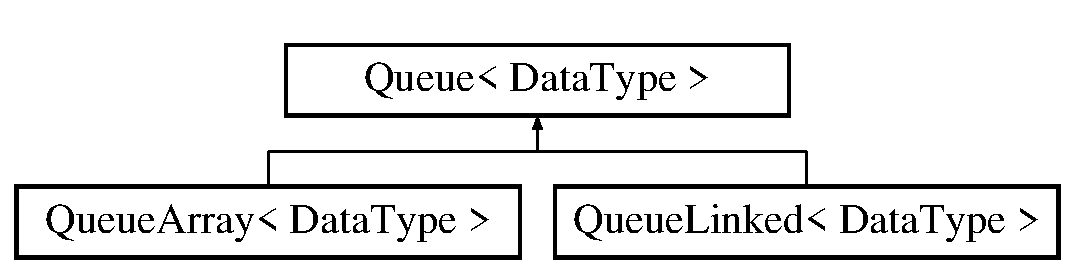
\includegraphics[height=2.000000cm]{class_queue}
\end{center}
\end{figure}
\subsection*{Public Member Functions}
\begin{DoxyCompactItemize}
\item 
virtual void {\bfseries enqueue} (const Data\+Type \&new\+Data\+Item)=0  throw (logic\+\_\+error)\label{class_queue_a4e0052bab8c2fb742a16a77d73ec3d5a}

\item 
virtual Data\+Type {\bfseries dequeue} ()=0  throw (logic\+\_\+error)\label{class_queue_afde1535196f515caba0aa5cfbe62d329}

\item 
virtual void {\bfseries clear} ()=0\label{class_queue_afba4d82c9a20859bb6397bd73c230cdd}

\item 
virtual bool {\bfseries is\+Empty} () const =0\label{class_queue_a1b8e1c0b8bb621de8d4f20c011176bd2}

\item 
virtual bool {\bfseries is\+Full} () const =0\label{class_queue_ae64751e270709a705d49e6168e64ade8}

\item 
virtual void {\bfseries show\+Structure} () const =0\label{class_queue_a44c7efe23657b7e1ed2ab1f815120eba}

\end{DoxyCompactItemize}
\subsection*{Static Public Attributes}
\begin{DoxyCompactItemize}
\item 
static const int {\bfseries M\+A\+X\+\_\+\+Q\+U\+E\+U\+E\+\_\+\+S\+I\+Z\+E} = 8\label{class_queue_aaf3eed0540baaf6609b48910aacc7133}

\end{DoxyCompactItemize}


The documentation for this class was generated from the following files\+:\begin{DoxyCompactItemize}
\item 
Queue.\+h\item 
show7.\+cpp\end{DoxyCompactItemize}

\section{Queue\+Array$<$ Data\+Type $>$ Class Template Reference}
\label{class_queue_array}\index{Queue\+Array$<$ Data\+Type $>$@{Queue\+Array$<$ Data\+Type $>$}}
Inheritance diagram for Queue\+Array$<$ Data\+Type $>$\+:\begin{figure}[H]
\begin{center}
\leavevmode
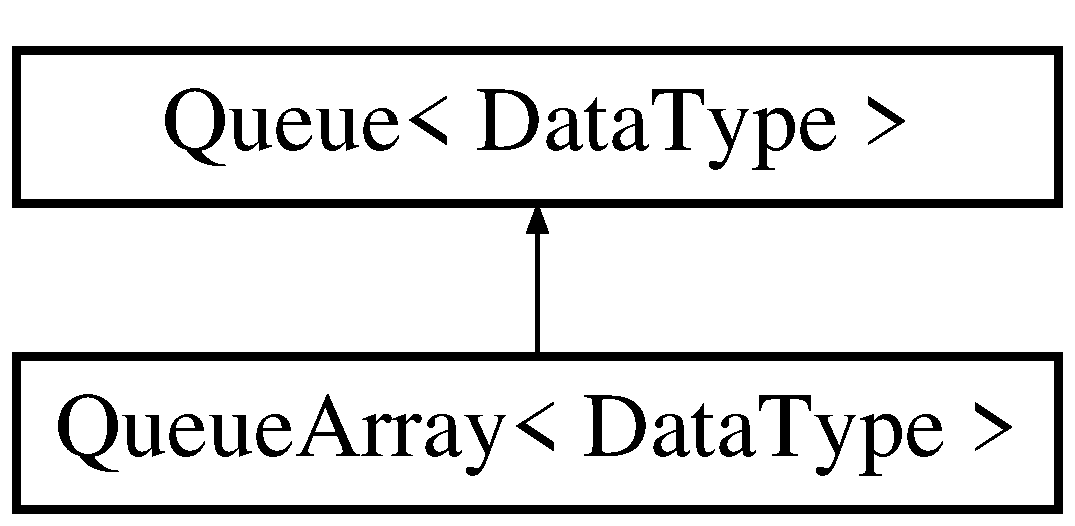
\includegraphics[height=2.000000cm]{class_queue_array}
\end{center}
\end{figure}
\subsection*{Public Member Functions}
\begin{DoxyCompactItemize}
\item 
{\bfseries Queue\+Array} (int max\+Number={\bf Queue}$<$ Data\+Type $>$\+::M\+A\+X\+\_\+\+Q\+U\+E\+U\+E\+\_\+\+S\+I\+Z\+E)\label{class_queue_array_a112114659f8c2590872426a2dee8e6cc}

\item 
{\bfseries Queue\+Array} (const {\bf Queue\+Array} \&other)\label{class_queue_array_a08df206def55e930c9c561ee8bc93422}

\item 
{\bf Queue\+Array} \& {\bfseries operator=} (const {\bf Queue\+Array} \&other)\label{class_queue_array_adaad55e5da06583cc786af90937a94c1}

\item 
void {\bfseries enqueue} (const Data\+Type \&new\+Data\+Item)  throw (logic\+\_\+error)\label{class_queue_array_a15e0632c580858c396d3aac1265fecd7}

\item 
Data\+Type {\bfseries dequeue} ()  throw (logic\+\_\+error)\label{class_queue_array_a34d386d2323aa80b7b441d4436153a89}

\item 
void {\bfseries clear} ()\label{class_queue_array_a154afbf4084cb08e3a134f2f6a33df6c}

\item 
bool {\bfseries is\+Empty} () const \label{class_queue_array_ae1298c7e16e1053b628a019e71db4320}

\item 
bool {\bfseries is\+Full} () const \label{class_queue_array_a7233d591dd81e9e3d3f6e4ad5631c81c}

\item 
void {\bfseries put\+Front} (const Data\+Type \&new\+Data\+Item)  throw (logic\+\_\+error)\label{class_queue_array_add18fcb931a244d56040a1f0a0c24a8f}

\item 
Data\+Type {\bfseries get\+Rear} ()  throw (logic\+\_\+error)\label{class_queue_array_a8bebf91214e116f74d4482bf9babee2d}

\item 
int {\bfseries get\+Length} () const \label{class_queue_array_a1d1bf41a4ca23c30f53296a0e0c5bf33}

\item 
void {\bfseries show\+Structure} () const \label{class_queue_array_adde651b7fd7865dc4f281e21c7f1a6c3}

\end{DoxyCompactItemize}
\subsection*{Additional Inherited Members}


The documentation for this class was generated from the following files\+:\begin{DoxyCompactItemize}
\item 
Queue\+Array.\+h\item 
show7.\+cpp\end{DoxyCompactItemize}

\section{Queue\+Linked$<$ Data\+Type $>$ Class Template Reference}
\label{class_queue_linked}\index{Queue\+Linked$<$ Data\+Type $>$@{Queue\+Linked$<$ Data\+Type $>$}}
Inheritance diagram for Queue\+Linked$<$ Data\+Type $>$\+:\begin{figure}[H]
\begin{center}
\leavevmode
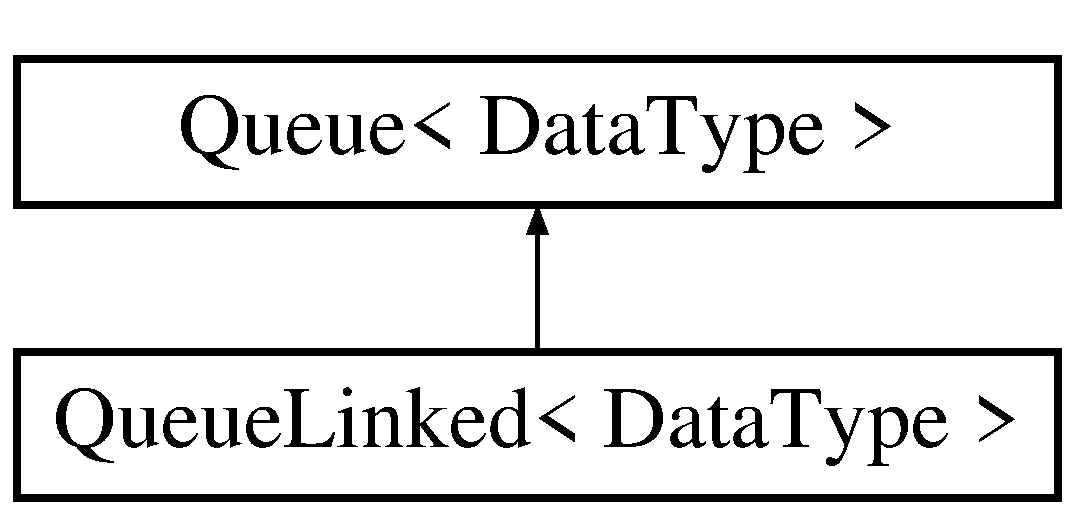
\includegraphics[height=2.000000cm]{class_queue_linked}
\end{center}
\end{figure}
\subsection*{Public Member Functions}
\begin{DoxyCompactItemize}
\item 
{\bf Queue\+Linked} (int max\+Number={\bf Queue}$<$ Data\+Type $>$\+::M\+A\+X\+\_\+\+Q\+U\+E\+U\+E\+\_\+\+S\+I\+Z\+E)
\item 
{\bf Queue\+Linked} (const {\bf Queue\+Linked} \&other)
\item 
{\bf Queue\+Linked} \& {\bf operator=} (const {\bf Queue\+Linked} \&other)
\item 
{\bf $\sim$\+Queue\+Linked} ()
\item 
void {\bf enqueue} (const Data\+Type \&new\+Data\+Item)  throw (logic\+\_\+error)
\item 
Data\+Type {\bf dequeue} ()  throw (logic\+\_\+error)
\item 
void {\bf clear} ()
\item 
bool {\bf is\+Empty} () const 
\item 
bool {\bf is\+Full} () const 
\item 
void {\bf put\+Front} (const Data\+Type \&new\+Data\+Item)  throw (logic\+\_\+error)
\item 
Data\+Type {\bf get\+Rear} ()  throw (logic\+\_\+error)
\item 
int {\bf get\+Length} () const 
\item 
void {\bf show\+Structure} () const 
\end{DoxyCompactItemize}
\subsection*{Additional Inherited Members}


\subsection{Constructor \& Destructor Documentation}
\index{Queue\+Linked@{Queue\+Linked}!Queue\+Linked@{Queue\+Linked}}
\index{Queue\+Linked@{Queue\+Linked}!Queue\+Linked@{Queue\+Linked}}
\subsubsection[{Queue\+Linked}]{\setlength{\rightskip}{0pt plus 5cm}template$<$class Data\+Type $>$ {\bf Queue\+Linked}$<$ Data\+Type $>$\+::{\bf Queue\+Linked} (
\begin{DoxyParamCaption}
\item[{int}]{max\+Number = {\ttfamily {\bf Queue}$<$DataType$>$\+:\+:MAX\+\_\+QUEUE\+\_\+SIZE}}
\end{DoxyParamCaption}
)}\label{class_queue_linked_ad356fca32ffd90c78d35d3eb5d84504b}
Method implementations This constructor creates an empty queue.


\begin{DoxyParams}{Parameters}
{\em int} & Max Number of data items this queue can hold \\
\hline
\end{DoxyParams}
\begin{DoxyReturn}{Returns}
This constructor does not return anything 
\end{DoxyReturn}
\begin{DoxyPrecond}{Precondition}
None 
\end{DoxyPrecond}
\begin{DoxyPostcond}{Postcondition}
Creates an empty queue. Allocates enough memory for the queue containing max\+Number data items if necessary) 
\end{DoxyPostcond}
\index{Queue\+Linked@{Queue\+Linked}!Queue\+Linked@{Queue\+Linked}}
\index{Queue\+Linked@{Queue\+Linked}!Queue\+Linked@{Queue\+Linked}}
\subsubsection[{Queue\+Linked}]{\setlength{\rightskip}{0pt plus 5cm}template$<$class Data\+Type $>$ {\bf Queue\+Linked}$<$ Data\+Type $>$\+::{\bf Queue\+Linked} (
\begin{DoxyParamCaption}
\item[{const {\bf Queue\+Linked}$<$ Data\+Type $>$ \&}]{other}
\end{DoxyParamCaption}
)}\label{class_queue_linked_ad8749850191f8a4165c8e3a3a266bada}
This copy constructor will make a deep copy of another queue. Initializes front and back to N\+U\+L\+L, then uses the enqueue method to add items from the other queue.


\begin{DoxyParams}{Parameters}
{\em Queue\+Linked\&} & Linked \doxyref{Queue}{p.}{class_queue} to copy \\
\hline
\end{DoxyParams}
\begin{DoxyReturn}{Returns}
This copy constructor does not return anything 
\end{DoxyReturn}
\begin{DoxyPrecond}{Precondition}
None 
\end{DoxyPrecond}
\begin{DoxyPostcond}{Postcondition}
Initializes the queue to be equivalent to the other \doxyref{Queue}{p.}{class_queue} object paramter 
\end{DoxyPostcond}
\index{Queue\+Linked@{Queue\+Linked}!````~Queue\+Linked@{$\sim$\+Queue\+Linked}}
\index{````~Queue\+Linked@{$\sim$\+Queue\+Linked}!Queue\+Linked@{Queue\+Linked}}
\subsubsection[{$\sim$\+Queue\+Linked}]{\setlength{\rightskip}{0pt plus 5cm}template$<$class Data\+Type $>$ {\bf Queue\+Linked}$<$ Data\+Type $>$\+::$\sim${\bf Queue\+Linked} (
\begin{DoxyParamCaption}
{}
\end{DoxyParamCaption}
)}\label{class_queue_linked_aed85fa73c60384a3d0c676c0ebbbca19}
Destructor. Deallocates the memory used to store the queue. Calls the clear method.

\begin{DoxyReturn}{Returns}
This destructor does not return anything 
\end{DoxyReturn}
\begin{DoxyPrecond}{Precondition}
None 
\end{DoxyPrecond}
\begin{DoxyPostcond}{Postcondition}
Deallocates the memory used to store the queue. 
\end{DoxyPostcond}


\subsection{Member Function Documentation}
\index{Queue\+Linked@{Queue\+Linked}!clear@{clear}}
\index{clear@{clear}!Queue\+Linked@{Queue\+Linked}}
\subsubsection[{clear}]{\setlength{\rightskip}{0pt plus 5cm}template$<$class Data\+Type $>$ void {\bf Queue\+Linked}$<$ Data\+Type $>$\+::clear (
\begin{DoxyParamCaption}
{}
\end{DoxyParamCaption}
)\hspace{0.3cm}{\ttfamily [virtual]}}\label{class_queue_linked_a32c66945765e5d42bbb988b1cdf43886}
Deletes all items in the queue, freeing memory and making the queue empty.

\begin{DoxyReturn}{Returns}
This method returns void. 
\end{DoxyReturn}
\begin{DoxyPrecond}{Precondition}
None. 
\end{DoxyPrecond}
\begin{DoxyPostcond}{Postcondition}
This queue will be empty 
\end{DoxyPostcond}


Implements {\bf Queue$<$ Data\+Type $>$} \doxyref{}{p.}{class_queue}.

\index{Queue\+Linked@{Queue\+Linked}!dequeue@{dequeue}}
\index{dequeue@{dequeue}!Queue\+Linked@{Queue\+Linked}}
\subsubsection[{dequeue}]{\setlength{\rightskip}{0pt plus 5cm}template$<$class Data\+Type $>$ Data\+Type {\bf Queue\+Linked}$<$ Data\+Type $>$\+::dequeue (
\begin{DoxyParamCaption}
{}
\end{DoxyParamCaption}
) throw  logic\+\_\+error) \hspace{0.3cm}{\ttfamily [virtual]}}\label{class_queue_linked_ac0656892f605af3b952c71706d3af55d}
If the queue is not empty, remove the first item in the queue (from the front) and return it. Otherwise, an error is thrown.

\begin{DoxyReturn}{Returns}
Data\+Type The first item in the queue 
\end{DoxyReturn}
\begin{DoxyPrecond}{Precondition}
\doxyref{Queue}{p.}{class_queue} is not empty 
\end{DoxyPrecond}
\begin{DoxyPostcond}{Postcondition}
Removes the least recently added data item from the queue and returns it. 
\end{DoxyPostcond}


Implements {\bf Queue$<$ Data\+Type $>$} \doxyref{}{p.}{class_queue}.

\index{Queue\+Linked@{Queue\+Linked}!enqueue@{enqueue}}
\index{enqueue@{enqueue}!Queue\+Linked@{Queue\+Linked}}
\subsubsection[{enqueue}]{\setlength{\rightskip}{0pt plus 5cm}template$<$class Data\+Type $>$ void {\bf Queue\+Linked}$<$ Data\+Type $>$\+::enqueue (
\begin{DoxyParamCaption}
\item[{const Data\+Type \&}]{new\+Data\+Item}
\end{DoxyParamCaption}
) throw  logic\+\_\+error) \hspace{0.3cm}{\ttfamily [virtual]}}\label{class_queue_linked_a7196448729d053f85f255674c7a57a02}
Inserts a new item to the back of the queue.


\begin{DoxyParams}{Parameters}
{\em Data\+Type\&} & Data to be inserted into the queue \\
\hline
\end{DoxyParams}
\begin{DoxyReturn}{Returns}
This function is void 
\end{DoxyReturn}
\begin{DoxyPrecond}{Precondition}
\doxyref{Queue}{p.}{class_queue} is not full 
\end{DoxyPrecond}
\begin{DoxyPostcond}{Postcondition}
Inserts new\+Data\+Item at the rear of the queue 
\end{DoxyPostcond}


Implements {\bf Queue$<$ Data\+Type $>$} \doxyref{}{p.}{class_queue}.

\index{Queue\+Linked@{Queue\+Linked}!get\+Length@{get\+Length}}
\index{get\+Length@{get\+Length}!Queue\+Linked@{Queue\+Linked}}
\subsubsection[{get\+Length}]{\setlength{\rightskip}{0pt plus 5cm}template$<$class Data\+Type $>$ int {\bf Queue\+Linked}$<$ Data\+Type $>$\+::get\+Length (
\begin{DoxyParamCaption}
{}
\end{DoxyParamCaption}
) const}\label{class_queue_linked_ab2d7fc0a927f3fe1e2ac44cc042bb961}
Counts and returns the number of items in the queue.

\begin{DoxyReturn}{Returns}
int Returns the number of items in the queue 
\end{DoxyReturn}
\begin{DoxyPrecond}{Precondition}
None 
\end{DoxyPrecond}
\begin{DoxyPostcond}{Postcondition}
The order and items in the queue will be unchanged. 
\end{DoxyPostcond}
\index{Queue\+Linked@{Queue\+Linked}!get\+Rear@{get\+Rear}}
\index{get\+Rear@{get\+Rear}!Queue\+Linked@{Queue\+Linked}}
\subsubsection[{get\+Rear}]{\setlength{\rightskip}{0pt plus 5cm}template$<$class Data\+Type $>$ Data\+Type {\bf Queue\+Linked}$<$ Data\+Type $>$\+::get\+Rear (
\begin{DoxyParamCaption}
{}
\end{DoxyParamCaption}
) throw  logic\+\_\+error) }\label{class_queue_linked_a2934f746096e31b9728de11f42bdc3cd}
Removes the last item from the queue and returns it.

\begin{DoxyReturn}{Returns}
Data\+Type Returns the last item in the queue 
\end{DoxyReturn}
\begin{DoxyPrecond}{Precondition}
\doxyref{Queue}{p.}{class_queue} is not empty. 
\end{DoxyPrecond}
\begin{DoxyPostcond}{Postcondition}
Removes the last item from the queue and returns it. 
\end{DoxyPostcond}
\index{Queue\+Linked@{Queue\+Linked}!is\+Empty@{is\+Empty}}
\index{is\+Empty@{is\+Empty}!Queue\+Linked@{Queue\+Linked}}
\subsubsection[{is\+Empty}]{\setlength{\rightskip}{0pt plus 5cm}template$<$class Data\+Type $>$ bool {\bf Queue\+Linked}$<$ Data\+Type $>$\+::is\+Empty (
\begin{DoxyParamCaption}
{}
\end{DoxyParamCaption}
) const\hspace{0.3cm}{\ttfamily [virtual]}}\label{class_queue_linked_a425b83383323217c924a41a0226f7022}
Returns true if the queue is empty. Otherwise, returns false.

\begin{DoxyReturn}{Returns}
bool Returns true if the queue has no items in it. 
\end{DoxyReturn}
\begin{DoxyPrecond}{Precondition}
None 
\end{DoxyPrecond}
\begin{DoxyPostcond}{Postcondition}
The queue will be unchanged 
\end{DoxyPostcond}


Implements {\bf Queue$<$ Data\+Type $>$} \doxyref{}{p.}{class_queue}.

\index{Queue\+Linked@{Queue\+Linked}!is\+Full@{is\+Full}}
\index{is\+Full@{is\+Full}!Queue\+Linked@{Queue\+Linked}}
\subsubsection[{is\+Full}]{\setlength{\rightskip}{0pt plus 5cm}template$<$class Data\+Type $>$ bool {\bf Queue\+Linked}$<$ Data\+Type $>$\+::is\+Full (
\begin{DoxyParamCaption}
{}
\end{DoxyParamCaption}
) const\hspace{0.3cm}{\ttfamily [virtual]}}\label{class_queue_linked_a3de199675ee629f9d20c48d0e2b65f71}
Returns true if the queue is full. Otherwise, returns false.


\begin{DoxyParams}{Parameters}
{\em } & return bool Always returns false. \\
\hline
\end{DoxyParams}
\begin{DoxyPrecond}{Precondition}
None. 
\end{DoxyPrecond}
\begin{DoxyPostcond}{Postcondition}
The queue will be unchanged 
\end{DoxyPostcond}


Implements {\bf Queue$<$ Data\+Type $>$} \doxyref{}{p.}{class_queue}.

\index{Queue\+Linked@{Queue\+Linked}!operator=@{operator=}}
\index{operator=@{operator=}!Queue\+Linked@{Queue\+Linked}}
\subsubsection[{operator=}]{\setlength{\rightskip}{0pt plus 5cm}template$<$class Data\+Type $>$ {\bf Queue\+Linked}$<$ Data\+Type $>$ \& {\bf Queue\+Linked}$<$ Data\+Type $>$\+::operator= (
\begin{DoxyParamCaption}
\item[{const {\bf Queue\+Linked}$<$ Data\+Type $>$ \&}]{other}
\end{DoxyParamCaption}
)}\label{class_queue_linked_acec147d4de2139d2b6fd511bca6d6299}
Overloaded assignment operator. Creates a deep copy of another linked queue by clearing the current list and then using the enqueue method to insert new items into the list.


\begin{DoxyParams}{Parameters}
{\em Queue\+Linked\&} & Other linked queue that this queue will be a copy of \\
\hline
\end{DoxyParams}
\begin{DoxyReturn}{Returns}
A reference to the modified queue 
\end{DoxyReturn}
\begin{DoxyPrecond}{Precondition}
None 
\end{DoxyPrecond}
\begin{DoxyPostcond}{Postcondition}
Sets the queue to be equivalent to the other \doxyref{Queue}{p.}{class_queue} object parameters and returns a reference to the modified queue 
\end{DoxyPostcond}
\index{Queue\+Linked@{Queue\+Linked}!put\+Front@{put\+Front}}
\index{put\+Front@{put\+Front}!Queue\+Linked@{Queue\+Linked}}
\subsubsection[{put\+Front}]{\setlength{\rightskip}{0pt plus 5cm}template$<$class Data\+Type $>$ void {\bf Queue\+Linked}$<$ Data\+Type $>$\+::put\+Front (
\begin{DoxyParamCaption}
\item[{const Data\+Type \&}]{new\+Data\+Item}
\end{DoxyParamCaption}
) throw  logic\+\_\+error) }\label{class_queue_linked_a838a51b8023f9cf3a5a24abb67ae1ee4}
Inserts a new data item to the front of the queue without changing the order of the original queue.


\begin{DoxyParams}{Parameters}
{\em Data\+Type\&} & A new item to add to the queue \\
\hline
\end{DoxyParams}
\begin{DoxyReturn}{Returns}
This function returns void. 
\end{DoxyReturn}
\begin{DoxyPrecond}{Precondition}
\doxyref{Queue}{p.}{class_queue} is not full 
\end{DoxyPrecond}
\begin{DoxyPostcond}{Postcondition}
new\+Data\+Item will be inserted at the front of the queue 
\end{DoxyPostcond}
\index{Queue\+Linked@{Queue\+Linked}!show\+Structure@{show\+Structure}}
\index{show\+Structure@{show\+Structure}!Queue\+Linked@{Queue\+Linked}}
\subsubsection[{show\+Structure}]{\setlength{\rightskip}{0pt plus 5cm}template$<$typename Data\+Type $>$ void {\bf Queue\+Linked}$<$ Data\+Type $>$\+::show\+Structure (
\begin{DoxyParamCaption}
{}
\end{DoxyParamCaption}
) const\hspace{0.3cm}{\ttfamily [virtual]}}\label{class_queue_linked_ab1a9a59860432f20b6c021a4dd2b1eb8}
Outputs the data items in the queue. If the queue is empty, outputs \char`\"{}\+Empty Queue\char`\"{}. This operation is intended only for testing/debugging purposes, and only supports queue data items that are one of C++'s predefined data types (int, char, etc) or other data structures with an overriden ostream operator$<$$<$.

\begin{DoxyReturn}{Returns}
This function returns void 
\end{DoxyReturn}
\begin{DoxyPrecond}{Precondition}
None 
\end{DoxyPrecond}
\begin{DoxyPostcond}{Postcondition}
The order and items in the queue will be unchanged. 
\end{DoxyPostcond}


Implements {\bf Queue$<$ Data\+Type $>$} \doxyref{}{p.}{class_queue}.



The documentation for this class was generated from the following files\+:\begin{DoxyCompactItemize}
\item 
Queue\+Linked.\+h\item 
{\bf Queue\+Linked.\+cpp}\end{DoxyCompactItemize}

\chapter{File Documentation}
\section{Queue\+Linked.\+cpp File Reference}
\label{_queue_linked_8cpp}\index{Queue\+Linked.\+cpp@{Queue\+Linked.\+cpp}}


This program will implement a Linked \doxyref{Queue}{p.}{class_queue}.  


{\ttfamily \#include \char`\"{}Queue\+Linked.\+h\char`\"{}}\\*


\subsection{Detailed Description}
This program will implement a Linked \doxyref{Queue}{p.}{class_queue}. 

\begin{DoxyAuthor}{Author}
Tim Kwist 
\end{DoxyAuthor}
\begin{DoxyVersion}{Version}
1.\+0
\end{DoxyVersion}
The specifications of this program are defined by C++ Data Structures\+: A Laboratory Course (3rd edition) by Brandle, J\+Geisler, Roberge, Whittington, exercise 7. This implementation only implements the Linked List version of the \doxyref{Queue}{p.}{class_queue}. \begin{DoxyDate}{Date}
Wednesday, September 10, 2014 
\end{DoxyDate}

%--- End generated contents ---

% Index
\newpage
\phantomsection
\addcontentsline{toc}{chapter}{Index}
\printindex

\end{document}
